El monitor TRITIUM presenta un disseny modular, és a dir, consta de diversos prototips, anomenats mòduls quan formen part del monitor, que són llegits en paral·lel. Un disseny esquemàtic del monitor format per $10$ mòduls TRITIUM-IFIC-2 es mostra a la Figura \ref{fig:10TritiumMonitorIFIC2}.
\begin{figure}[h]
\centering
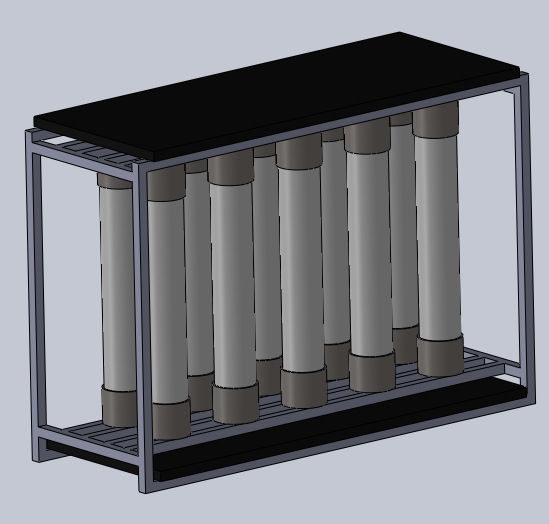
\includegraphics[scale=0.6]{12Summary/5Prototypes/55ModularTritiumDetector/Tritium_Detector_Based_On_Tritium_IFIC_2.PNG}
\caption{Disseny esquemàtic del monitor TRITIUM basat en el prototip TRITIUM-IFIC-2.\label{fig:10TritiumMonitorIFIC2}}
\end{figure}
Aquesta modularitat és una de les propietats més rellevants del monitor, ja que li confereix la possibilitat de millorar algunes de les seues característiques de forma proporcional al nombre de mòduls. Una de les propietats més rellevants per al projecte TRITIUM és la mínima activitat de triti detectable pel monitor (MDA), la millora del qual varia de forma proporcional a l'arrel del nombre de mòduls. La Figura \ref{fig:MDATritiumMonitorIFIC2} mostra el comportament esperat del MDA per al monitor TRITIUM basat en el prototip TRITIUM-IFIC-2 en funció del nombre de mòduls. La línia de color roig mostra l'objectiu de la col·laboració TRITIUM de $100~\becquerel/\liter$. Com es pot veure, s'espera aconseguir aquest objectiu amb $5$ mòduls TRITIUM-IFIC-2 llegits en paral·lel.

\begin{figure}[h]
\centering
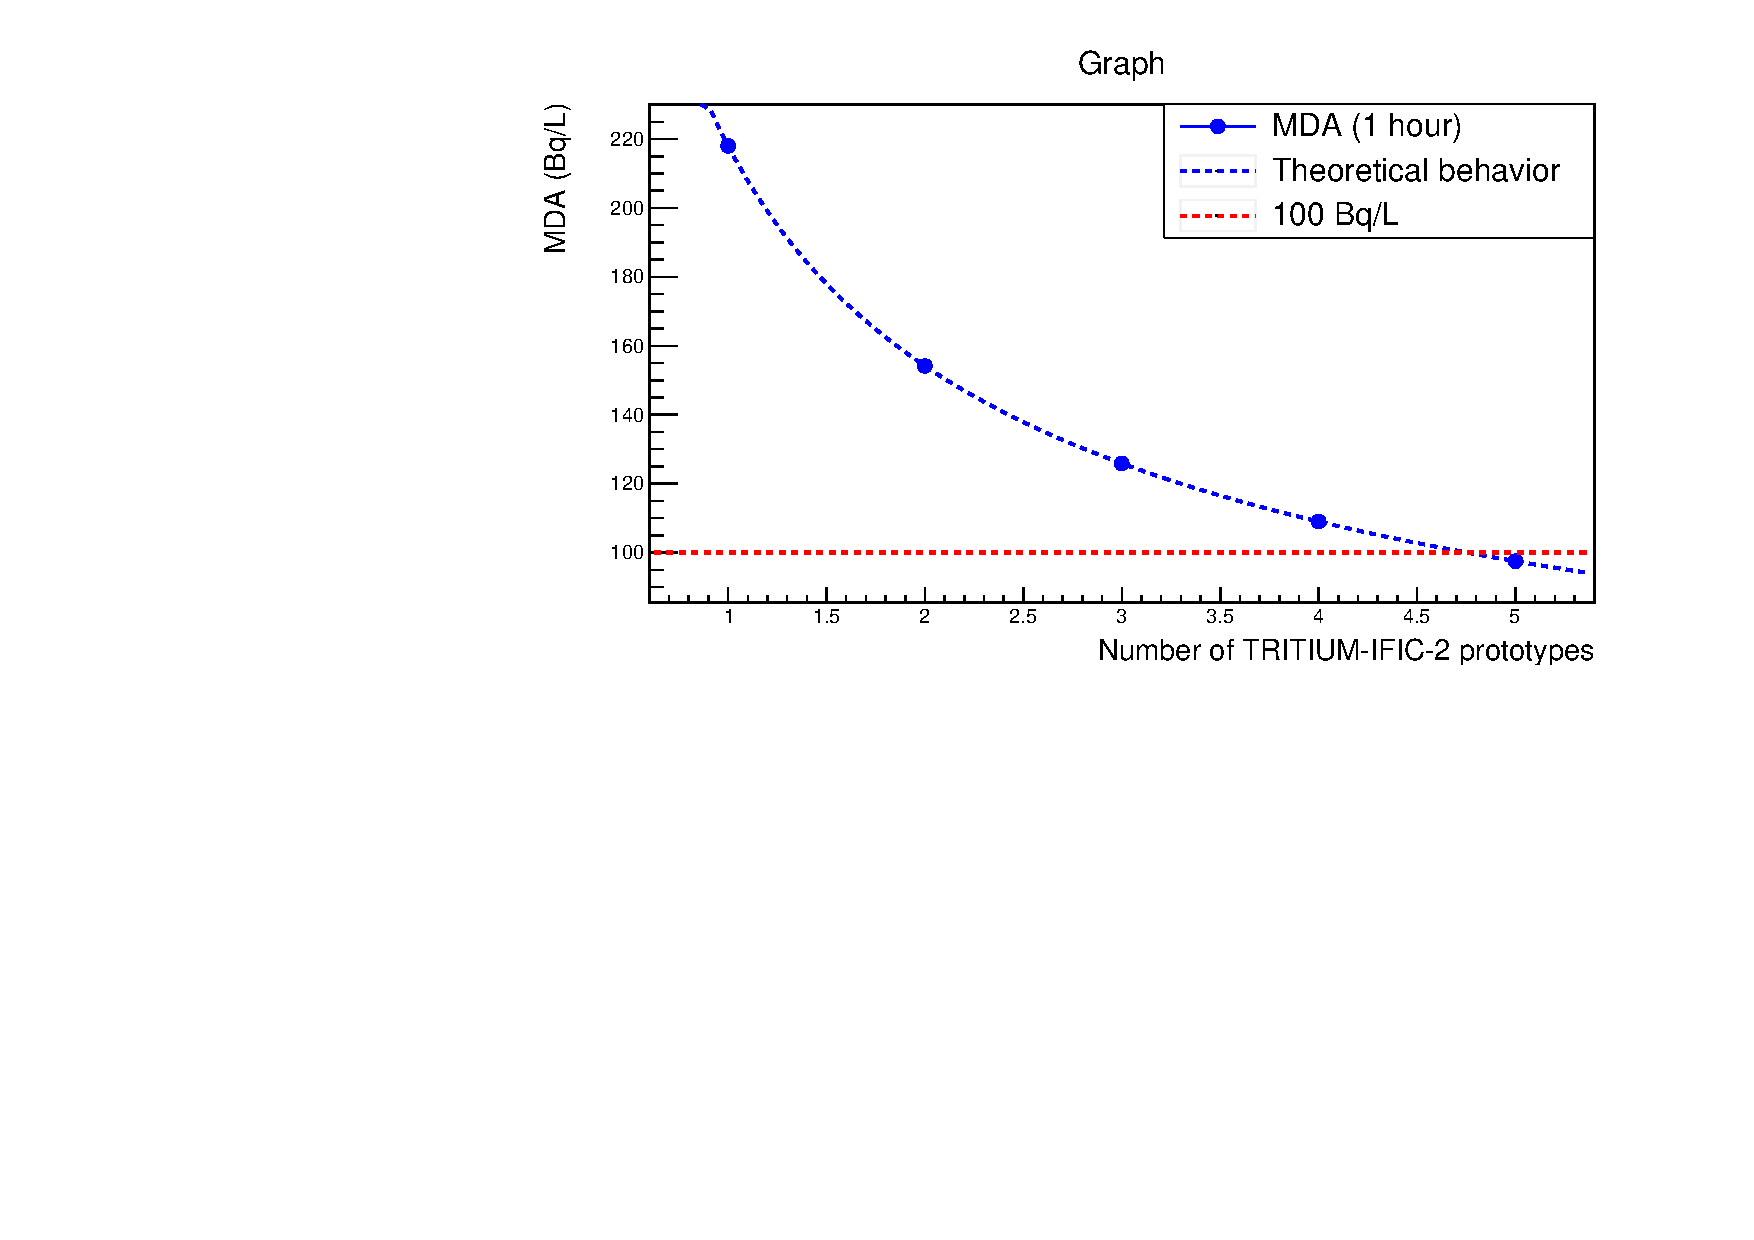
\includegraphics[scale=0.6]{12Summary/5Prototypes/55ModularTritiumDetector/MDA_vs_NP.pdf}
\caption{Mínima activitat de triti detectable pel monitor TRITIUM en funció dels mòduls TRITIUM-IFIC-2 utilitzats.\label{fig:MDATritiumMonitorIFIC2}}
\end{figure}

Amb l'ajuda de simulacions es va estudiar com varia la resolució del monitor en funció del nombre de mòduls, paràmetre que indica la mínima variació de l'activitat de triti que som capaços d'identificar. Com es pot observar a la Figura \ref{fig:ResolucioTritiumMonitorIFIC2},  resolucions més baixes són obtingudes quan més mòduls són utilitzats, permetent diferenciar variacions més xicotetes en l'activitat de la mostra. Amb la utilització de $5$ mòduls TRITIUM-IFIC-2 llegits en paral·lel s'aconsegueix identificar correctament variacions en l'activitat del triti de $100~\becquerel/\liter$ en mesures de $1~\hour$.

\begin{figure}[h]
\centering
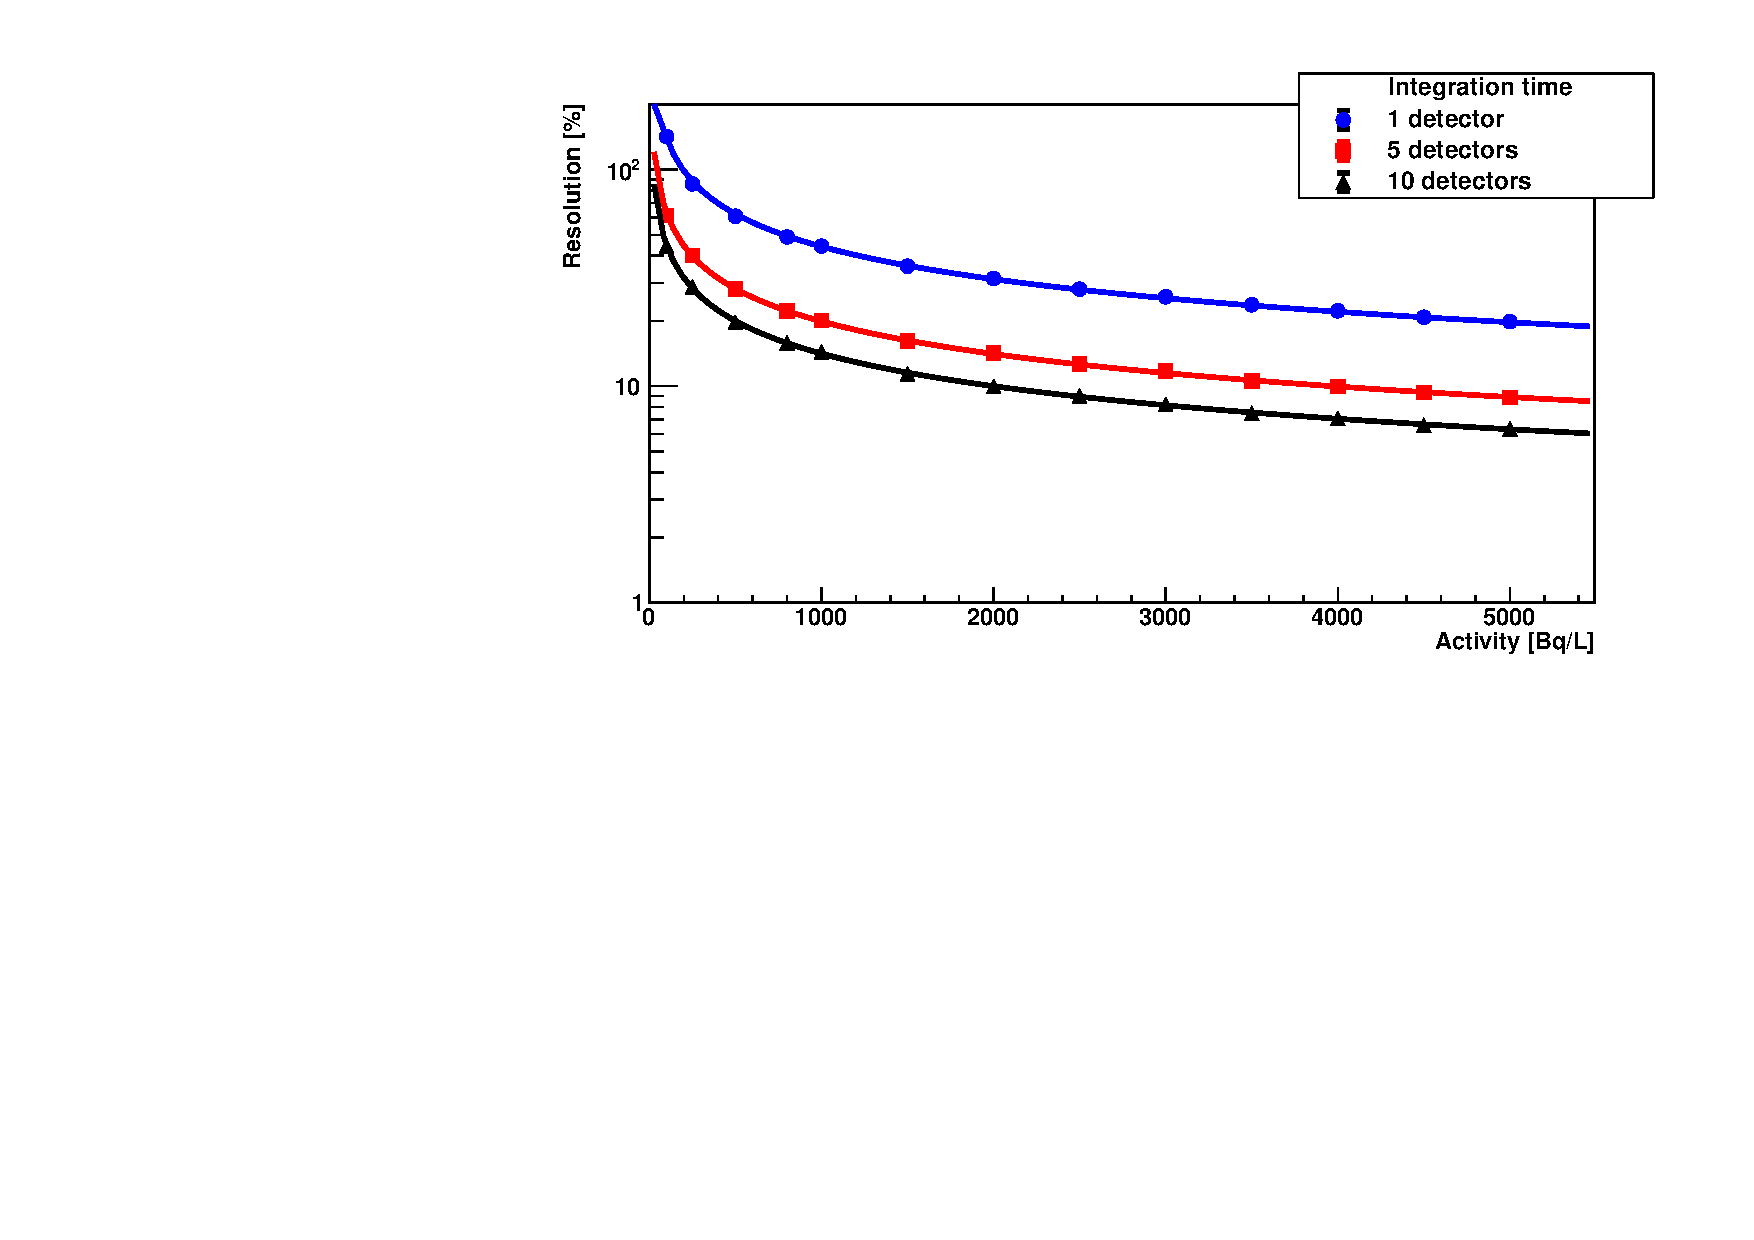
\includegraphics[scale=0.6]{12Summary/6Simulations/62TRITIUMMonitor/621TRITIUMIFIC2/Results_Several_Detectors.pdf}
\caption{Resolució monitor TRITIUM basat en mòduls TRITIUM-IFIC-2 en funció del nombre de mòduls.\label{fig:ResolucioTritiumMonitorIFIC2}}
\end{figure}